% !TEX TS-program = pdflatex
% !TEX encoding = UTF-8 Unicode

% This is a simple template for a LaTeX document using the "article" class.
% See "book", "report", "letter" for other types of document.

\documentclass[12pt]{article} % use larger type; default would be 10pt

\usepackage[utf8]{inputenc} % set input encoding (not needed with XeLaTeX)

%%% Examples of Article customizations
% These packages are optional, depending whether you want the features they provide.
% See the LaTeX Companion or other references for full information.

%%% PAGE DIMENSIONS
\usepackage{geometry} % to change the page dimensions
\geometry{a4paper} % or letterpaper (US) or a5paper or....
% \geometry{margin=2in} % for example, change the margins to 2 inches all round
% \geometry{landscape} % set up the page for landscape
%   read geometry.pdf for detailed page layout information

\usepackage{graphicx} % support the \includegraphics command and options

% \usepackage[parfill]{parskip} % Activate to begin paragraphs with an empty line rather than an indent

%%% PACKAGES
\usepackage{booktabs} % for much better looking tables
\usepackage{array} % for better arrays (eg matrices) in maths
\usepackage{paralist} % very flexible & customisable lists (eg. enumerate/itemize, etc.)
\usepackage{verbatim} % adds environment for commenting out blocks of text & for better verbatim
\usepackage{subfig} % make it possible to include more than one captioned figure/table in a single float
% These packages are all incorporated in the memoir class to one degree or another...

%%% HEADERS & FOOTERS
\usepackage{fancyhdr} % This should be set AFTER setting up the page geometry
\pagestyle{fancy} % options: empty , plain , fancy
\renewcommand{\headrulewidth}{0pt} % customise the layout...
\lhead{}\chead{}\rhead{}
\lfoot{}\cfoot{\thepage}\rfoot{}

%%% SECTION TITLE APPEARANCE
\usepackage{sectsty}
\usepackage{helvet}
\usepackage{titlesec}
\usepackage{inputenc}
\usepackage{amsmath}
\allsectionsfont{\sffamily\mdseries\upshape} % (See the fntguide.pdf for font help)
\titleformat{\section}
{\normalfont\fontsize{16}{19}\sffamily\bfseries}
{\thesection}
{1em}
{}

\titleformat{\subsection}
{\normalfont\fontsize{12}{17}\sffamily\bfseries}
{\thesubsection}
{1em}
{}

\titleformat{\subsubsection}
{\normalfont\fontsize{12}{17}\sffamily\bfseries}
{\thesubsubsection}
{1em}
{}
% (This matches ConTeXt defaults)

%%% ToC (table of contents) APPEARANCE
\usepackage[nottoc,notlof,notlot]{tocbibind} % Put the bibliography in the ToC
\usepackage[titles,subfigure]{tocloft} % Alter the style of the Table of Contents
\renewcommand{\cftsecfont}{\rmfamily\mdseries\upshape}
\renewcommand{\cftsecpagefont}{\rmfamily\mdseries\upshape} % No bold!

%%% END Article customizations

%%% The "real" document content comes below...

%\date{} % Activate to display a given date or no date (if empty),
         % otherwise the current date is printed 
\usepackage{url}
\usepackage{float}
\usepackage{indentfirst}

\setcounter{tocdepth}{3}

\graphicspath {{Resources/}}

%\setlength{\parindent}{4em}

\begin{document}
\input{"title_page.tex"}
\tableofcontents
\newpage
\listoffigures
\newpage
\listoftables
\newpage

\newpage
\section{Introduction}
Music is universal and it's significance is nothing to mess about. Every known civilization has a form of music. From baroque, classical, opera, jazz, traditional folk, rock, rap or contemporary pop music, the sharing of music provides endless joy for humans.
\par
Music transcription is defined as the task of converting music from sound into a written, abstract notation.
It is the inverse operation of music performance, which often involves a performer reading music notation and producing sound waves with the help of an instrument or their voice. Because music is an universal language people around the globe can share music with each other surpassing the language barrier.
\par
Manual music transcription is a task difficult enough that even the best musicians struggle to achieve 100\% accuracy. It takes a lot of time and practice to learn and even more to master. In order to facilitate the process and make transcription available to everyone people tried to figure out ways to automate the process. It was at this moment, in 1977, Automatic music transcription (AMT) was born.
\par
For the past decades, this field of computer science research has been developing and still has numerous unsolved problems. Every year shows new research with improved algorithms for various sub tasks of AMT.
\par
The goal of this thesis is to introduce the field of automatic music transcription and provide a deep learning approach to pitch estimation using convolutional neural networks (CNNs).

\newpage
\section{Theoretical Background}
\subsection{Introduction to Deep Learning}
\vspace{1em}
Machine learning (ML) is the scientific study of algorithms and statistical models that computer systems use to effectively perform a specific task without using explicit instructions, relying on patterns and inference instead. Machine learning algorithms build a mathematical model of sample data, known as "training data", in order to make predictions or decisions without being explicitly programmed to perform the task. Machine learning algorithms are used in a wide variety of applications, such as email filtering, and computer vision, where it is infeasible to develop an algorithm of specific instructions for performing the task. The represantation of data fed into a ML algorithm plays a major role, as it affects the algorithm’s ability to efficiently extract signals and make decisions. Thus, it is important to carefully select the information included in such a representation. Formally, the representation is com- posed of multiple features extracted from raw data. The process of creating new features requires good and intuitive understanding of the data at hand, becoming incrementally time-consuming with the sophistication of the new features. Thus, the biggest challenge of handcrafted features is deciding which features are important and relevant to the problem \cite{Goodfellow-et-al-2016}\par



\section{Neural Networks}
This section introduces the main concepts related to neural networks. Neural networks have been around since the 1940s and could initially handle only one hidden layer. But with the development of technologies and hardware, it became possible to build deeper, more effective architectures, which lead to deep learning as we know it today. \par



\subsection{Brief History}


At first, neural networks were inspired by the functioning of the biological brain, which is why deep learning is also called artificial neural networks (ANNs)~\cite{Goodfellow-et-al-2016}. In biology, a neuron is the cell that receives, processes and transmits information to other neurons through connections called synapses~\cite{neuron}. On the other hand, artificial neurons are defined as computational units (usually mathematical functions) that take one or more inputs and generate an output. \par

McCulloch and Pits designed an initial version of the neuron as a linear model in 1943, aiming to replicate brain function~\cite{REF:11}:


\begin{equation}
f(x,w)=x_1*w_1 +x_2*w_2 +...+x_n*w_n
\end{equation}
where $x_1, ..., x_n$ are the input values and $w_1, ..., w_2$ is a set of hand-chosen weights.

\subsection{Components of an artificial neural network}

A simple artificial neural network (ANN) consists of an input layer, hidden layer and output layer, where the values of the hidden layer are used as inputs for the output layer. A network with several layers is known as a deep neural network. Data flows through the neurons of the layer. Each neuron transforms the input it receives and sends it to the next layer. The neurons share the same characteristics regardless of the layer they are part of. \par



The Neuron, also called a node, is the basic unit of a neural network. Its main components include inputs,
weights, activation function and output(s). From a high-level point of view, the inputs are multiplied by 
weights, then an activation function is applied to the result and finally, another function computes the output~\cite{REF:12}~\cite{REF:13}. \par


\begin{itemize}
	\item Weights are defined as adaptive coefficients, whose values are changed during the learning process. They represent the strength of the connection between units. A weight decides how much impact the input will have on the output
	
	\item The summation function helps combine the input and weights, before passing the result to the activation function. Denote the input as $X = [x_1, x_2, ...x_n]$ and the weight vector as $W = [w_1, w_2, ...w_n]$.\\
	The summation function could be defined as the dot product between these two vectors:\\
	\begin{equation}
	X \cdot W =x_1 \cdot w_1 +x_2 \cdot w_2 +...+x_n \cdot w_n
	\end{equation}

	
	The summation function could instead compute the minimum, maximum, etc. depending on the designated network architecture. The simplest form of an artificial neuron is a linear function which computes the weighted sum of inputs, to which, optionally, bias can be added:
	\begin{equation}
		y = \sum_{i=1}^{i=n}(x_i \cdot w_i) + b \textnormal{, where $b$ is the bias, $x_i \in X, w_i \in W$}
	\end{equation}

	
	\item The activation function transforms the result of the summation function (usually) in a non-linear way. Typically, it has a squashing effect. It serves as a threshold. It divides the original space into two partitions. Its main purpose is to make the neural network non-linear. We denote the activation function as $g$
	\begin{equation}
		y = g(\sum_{i=1}^{i=n}(x_i \cdot w_i) + b) \textnormal{, where $b$ is the bias, $x_i \in X, w_i \in W$}
	\end{equation}

	
	\begin{figure}[h]
		\caption[Common activation functions]{Common activation functions~\cite{activation_fig} }
		\centering
		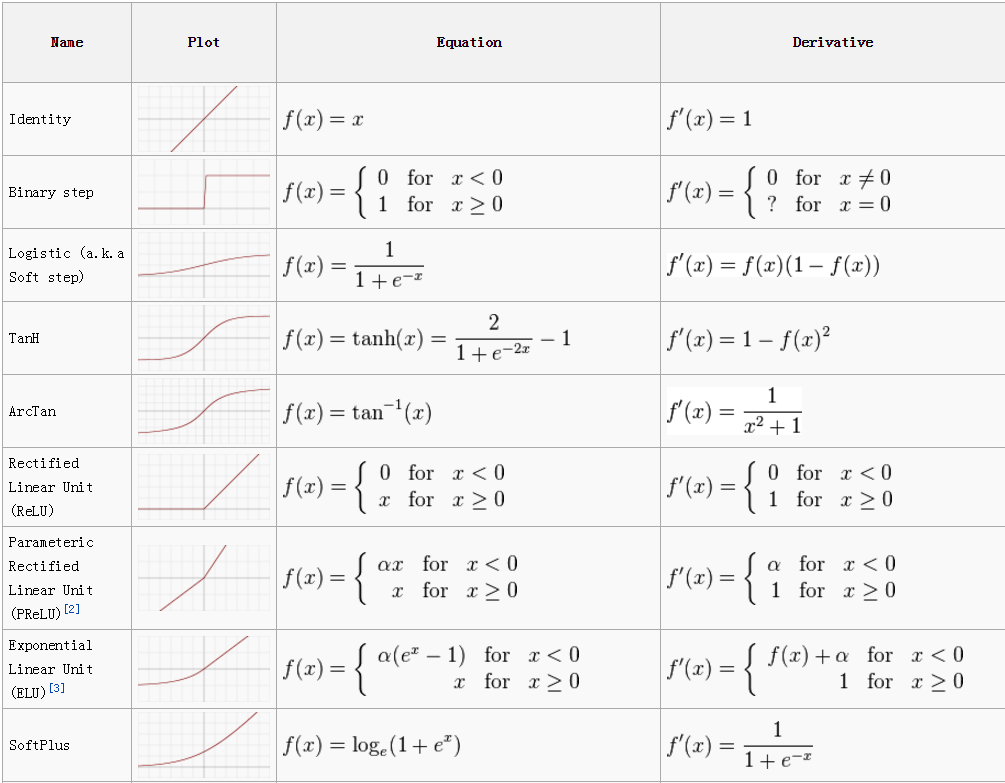
\includegraphics[width=1\textwidth, height=\textheight, keepaspectratio]{activation}
	\end{figure}
	\item The output is usually the result of an activation function
	
\end{itemize}

\clearpage
\subsection{Under-fitting and Over-fitting}
%reformulat + surse noi

Neural networks are able to learn complicated non-linear functions to fit any training set. On the downside, this may lead to over-fitting where the neural network learns the training data so well that it is unable to generalize on new, unseen data. This problem can especially occur on datasets with a small amount of data to learn from. \par

Under-fitting, the counterpart of over-fitting, happens when a machine learning model isn’t complex enough to accurately capture relationships between a dataset’s features and a target variable. Under-fitted models result in problematic outcomes on new data or data that they  were not trained on, and many times perform poorly even on training data. \par


\begin{figure}[h]
	\caption[Example of over-fitting and under-fitting]{Example of over-fitting and under-fitting~\cite{vitaflux}}
	\centering
	\includegraphics[width=1\textwidth, height=\textheight, keepaspectratio]{"resources/overfitting"}
\end{figure}

\subsection{Convolutional Neural Networks}
\par
Convolutional Neural Networks (CNNs) are a class of Deep Neural Networks,
specialized in analyzing images. Their development was inspired by biological processes.
The connectivity pattern between neurons resembles the animal visual cortex~\cite{cnn}. \par

\begin{figure}[h]
	\centering
	\caption[Typical convolutional neural network architecture]{Typical CNN architecture~\cite{cnn_fig}}
	\label{fig:cnn}
	\includegraphics[width=1.1\textwidth, height=1.5\textheight, keepaspectratio]{"resources/typical_cnn"}
\end{figure}

\par
A convolutional neural network consists of an input and an output layer, as well as multiple hidden layers. The hidden layers are typically convolutional layers, RELU layers, pooling layers, fully connected layers and normalization layers~\cite{cnn_git}.

\begin{itemize}
	\item \textbf{Convolutional} layers are the core building block of convolutional networks. They are responsible for feature extraction and do most of the computation
	\item \textbf{Pooling} layers reduce the dimension of the data by combining the outputs of neuron clusters at one layer into a single neuron in the next layer
	\item \textbf{Normalization} layers apply a transformation that maintains the mean activation close to 0 and the activation standard deviation close to 1
	\item \textbf{Fully connected} layers link every neuron in one layer to every neuron in another layer
	\item \textbf{Dropout} layers have a \% chance to deactivate the neurons of a particular layer. This is a technique used to improve over-fitting by improving generalization. Forcing neurons to deactivate forces the network to learn the same "concept" with different neurons. It is mostly used after fully connected or pooling layers
\end{itemize}




\newpage
\subsection{Convolutional Neural Networks}
\par
Convolutional Neural Networks (CNNs) are a class of Deep Neural Networks,
specialized in analyzing images. They were inspired by biological processes.
The connectivity pattern between neurons resembles the animal visual cortex.
\cite{cnn} \par

\subsubsection{Find subsections}


\newpage



\newpage
\subsection{Music Transcription}
In music, transcription is the process of creating a music sheet from a piece or sound. The sheet contains music notation, which consists of different symbols that can be interpreted by musicians, hence it is important for various reasons. Without it composers such as Mozart and Beethoven couldn't have passed their masterpieces across generations. In modern days it helps musicians play songs they never heard before. It's also universal so even if two musicians don't speak the same language, they can read the same notation.

\subsubsection{Traditional Music Transcription}
In the beginning transcription was done by humans. It's also called musical dictation in ear training pedagogy. \cite{human_transcription} It is a skill by which musicians learn to identify pitches, intervals, melody, chords and other elements of music solely by hearing. It is a really hard skill, requires serious training and study and even the best don't have 100\% accuracy. \par

There are some tools to help with the process:
\begin{itemize}
	\item Musical instruments, help musicians test for certain sounds, trying to mimic what they hear
	\item Tape recorders
	\item Nowadays software
\end{itemize}

\subsubsection{Automated Music Transcription}
The term "Automated Music Transcription" was used for the first time in 1977, by audio researchers James A. Moorer, Martin Piszczalski, and Bernard Galler \cite{transcription}. With their knowledge about digital engineering they believed that computers could be programmed to analyze digital recordings of songs such that they could identify things like rhythm, melodies, pitch, bass lines. It's not an easy task. For more than three decades researchers have been trying to crack it open. \par

Fundamentally, AMT is about identifying the pitch and duration of played notes, so they can be converted in traditional music notation on a sheet. \par

It has many advantages over traditional transcription:
\begin{itemize}
	\item Aids experienced musicians in the process of transcribing pieces, increasing their accuracy.
	\item Makes music transcription available to more people, especially beginners, giving them a chance to share their ideas with others.
	\item Helps people learn new songs. There are a lot of music sheets online that are not free. 
	\item It speeds up the process. Manual transcription takes a lot of time.
\end{itemize}

\newpage
\section{Related Work}

Automatic music transcription (AMT) has been attempted since the 1970s and polyphonic music transcription dates to the 1990s \cite{REF:1}
\par

\subsection{State of the art in AMT}

There has been substantial progress made in the field of AMT. Neural networks, in particular, have met and surpassed the performance of traditional pitch recognition techniques on polyphonic audio.
\par

A model used in \cite{REF:2} uses 87 Support Vector Machine (SVM) classifiers to perform frame-level classification with the advantage of simplicity, and then a Hidden Markov Model (HMM) post-processing was adopted to smooth the results. On top of it, Deep Belief Network(DBN) was added to learn higher layer representation of features in \cite{REF:3}. Since none of the approaches has reached the same level of accuracy as human experts, most music transcription work is completed by musicians. With the development of deep learning in recent years, many researchers were inspired to apply networks to accomplish AMT. A model based on Convolutional Neural Networks (CNN) was proposed in \cite{REF:4}. More models adopted Reccurent Neural Networks (RNN) or Long Short-Term Memory (LSTM) due to its capability of dealing with sequential data \cite{REF:1} \cite{REF:5} \cite{REF:6}. In \cite{REF:7}, 5 models were compared and the ConvNet model was reported as resulting in the best performance.
\par

The first majort AMT work is Smaragdis et al.\cite{REF:8}. This approach uses Non-Negative Matrix Factorization (NMF). This is the main methodology employed in software for automatic transcription, but it has it's limitations. For example, it needs to know how many individual notes are desired for the transcription (information that is not always available).
\par

The next work worth mentioning is Emiya et al.\cite{REF:9}, not because of their transcription system (as it was out-performed in the same year), but because of the dataset they created that has become the standard in evaluating any multi-pitch estimation system. They created the MIDI-Aligned Piano Sounds (MAPS) data set composed of around 10,000 piano sounds either recorded by using an upright Disklavier piano or generated by several virtual piano software products based on sampled sounds. The dataset
consists of audio and corresponding annotations for isolated sounds, chords, and complete pieces of piano music.
\par

Sigtia et al.\cite{REF:10} built the first AMT system using CNN, outperforming the state of the art approaches using NMF. Convolutional
Neural Networks are a discriminative approach to AMT, which has been found to be a
viable alternative to spectrogram factorization techniques. Discriminative approaches
aim to directly classify features extracted from frames of audio to the output pitches.
This approach uses complex classifiers that are trained using large amounts of training
data to capture the variability in the inputs, instead of constructing an instrument
specific model. 
\par

Sigtia et al. \cite{REF:10} explored various models for pitch detection. In addition to CNNs, they tried Deep Neural Networks and Recurrent Neural Networks. The results have shown that their CNN based model outperformed the others for this task. In their paper, they propose a Music Language Model (MLM) that's based on RNNs in order to handle the polyphonic musical data. \cite{benetos}
\par

There are some products on the market, AnthemScore for example, that use CNNs for AMT. They approach note detection as an image recognition problem by creating spectrograms of the audio. They show how the spectrum or frequency content changes over time. The method used for creating the spectrograms is the constant Q transform instead of the more common Short Time Fourier Transform (STFT) method.
\par

Melodyne is a popular plugin used for Music Transcription and Pitch Correction. It costs up to \$700. 	
The Melodic and Polyphonic algorithms offer you, in the case of vocals as well as both mono- and polyphonic instruments, full access to the notes of which the sound is composed as well as to their musical parameters.
There's no public information about what approach they used.
\par

\subsection{CNN approach to AMT}




\newpage
\section{Application}

\section{Problem statement}
Automatic music transcription consists of analyzing digital recordings of songs and identify things like rhythm, melodies, pitch, bass lines. The main subtasks of AMT are:

\begin{itemize}
	\item \textbf{Pitch estimation}
	\item \textbf{Beat detection}
	\item \textbf{Instrument detection}
\end{itemize}

Because of the polyphonic approach of music, AMT is still unresolved today. The state of the art approaches struggle to get an accuracy greater than 70\%. It's a problem that requires a lot of digital signal processing knowledge in order to optimize the data and split the subtask even further in onset and offset detection, genre detection and velocity detection. In order to have a full prediction, you need to cover all of these tasks.
	
The proposed solution attempts the \textbf{Pitch estimation} part of AMT, using a heuristic approach to find the beat and creating spectrograms of the audio in order to get the instrument out of the equation.
	

Fundamentally, AMT is about identifying the pitch and duration of played notes, so they can be converted in traditional music notation on a sheet

\section{Data set and input representation}
The data set used was the MAPS database~\cite{maps}. It is a piano database for multi-pitch estimation and automatic transcription of music. It contains MIDI-annotated piano recordings, composed of isolated notes, random-pitch chords, usual musical chords and pieces of music. It provides a diverse range of sounds from various recording conditions.
\par
The recordings are CD quality (16-bit, $44-kHz$ sampled stereo audio) and the related aligned MIDI files contain the ground truth. The overall size of the database is 40GB. 
\par
Working with sound in neural networks is different from dealing with images. The input contains audio files so before feeding it to the network we need to turn it into a visual representation. The most common way to represent a sound is the audio representation in the time domain. (Figure \ref{fig:waveform})

\begin{figure}[h!]
	\caption[Example of audio representation in the time domain]{ Example of audio representation in the time domain~\cite{genre_class} }
	\centering
	\label{fig:waveform}
	\includegraphics[width=1\textwidth, height=\textheight, keepaspectratio]{"resources/waveform"}
\end{figure}

Figure \ref{fig:waveform} shows the evolution in time of the song and you can see the oscillation of the signal. The $Y$ axis represents the amplitude while the $X$ axis is the time. In this representation, it's not possible to distinguish the notes that are playing. Because of this, we need a better representation. This is where the Fourier Transformations come in handy. Using the transformation on the data we get a representation over frequency instead of time. This is also known as a spectrum. The spectrum reveals relevant information that's crucial to analyze the audio. (Figure \ref{fig:cq_vs_stft})
\par

The input MIDI file will be split into $\frac{1}{16}\cdot second$ window frames. For example, a note lasting 1 second will have 16 consecutive windows created. Each window is then turned into a .wav file, using fluidsynth~\cite{fluidsynth}, which in turn will be transformed using the Constant-Q transform.
One window transformation takes ~0.3 seconds making the process slow and punishing if a bug is found in the preprocessing.

\par
To compute the Constant-Q transform, the library \textit{Librosa}~\cite{librosa} will be used, in particular, the method called \textit{librosa.cqt}.
The parameters that we will use are:
\begin{itemize}
	\item \textbf{y}: Audio signal
	\item \textbf{sr}: Sampling rate
	\item \textbf{fmin}: Minimum frequency
	\item \textbf{n\_bins}: Number of frequency bins
	\item \textbf{bins\_per\_octave}: Number of bins per octave
	\item \textbf{hop\_length}: Number of samples between successive CQT columns
\end{itemize}
\par

The result of the Librosa function will be plotted, resulting in a logarithmic scale spectrogram of size $145\times49$ (Figure \ref{fig:q_spec}). This way from a song of length $x$, $x \cdot 16$ spectrograms will be extracted. These are the input of the network.  
	
\begin{figure}[H]
	\caption[Example of a constant-q spectrogram]{ Example of a constant-q spectrogram }
	\centering
	\label{fig:q_spec}
	\includegraphics[width=1\textwidth, height=\textheight, keepaspectratio]{"resources/q_spec"}
\end{figure}

\par

For the cross validation, a train-validation-test split approach was used. The learning set was split $80\%$ for training, $20\%$ for testing and $10\%$ of the training set is used for validation. A visual representation can be seen in Figure \ref{fig:split}


\begin{figure}[H]
	\caption[Visual representation of the split]{ Visual representation of the split}
	\centering
	\label{fig:split}
	\includegraphics[width=1\textwidth, height=\textheight, keepaspectratio]{"resources/train_split"}
\end{figure}


\section{Labeling}
A supervised machine learning model needs the data to be labeled. As it was explained in the subsection above, the input song is going to be represented in the frequency domain. The labeling will be provided using the MIDI files associated with the input \textit{.wav} files. They contain information about the notes playing at a certain time. The labels will be arrays showing the played notes represented with \textit{one-hot encoding}.
\par

One-hot encoding is a widely used technique in neural networks. It consists of creating an array of boolean values~\cite{one-hot}. In this case, every column symbolizes a possible note that can be played at a certain moment. Because of this, there are as many columns as possible notes (128). This will be done per window, so the goal is to see which notes are played in a certain window (Table \ref{table:one_hot}). A value of 1 in a cell means that the specific musical note has been played during that window, while a value of 0 is the opposite.

\begin{table}
	\centering
	\caption{Example of one hot representation of a MIDI file}
	\begin{tabular}{||c c c c c||} 
		\hline
		Note & Window 1 & Window 2 & ... & Window n \\ [0.5ex] 
		\hline\hline
		1 & 0 & 0 & ... & 0 \\ 
		\hline
		2 & 1 & 0 & ... & 0 \\
		\hline
		3 & 0 & 0 & ... & 1 \\
		\hline
		... & ... & ... & ... & ... \\
		\hline
		128 & 0 & 1 & ... & 0 \\ [1ex] 
		\hline
	\end{tabular}
	\label{table:one_hot}
\end{table}

\section{First CNN architecture}
The first neural network has been created with the aim of obtaining some initial results and it has served to learn how a model developed in Keras~\cite{keras} behaves.
\par
An architecture similar to the Keras MNIST is evaluated~\cite{keras_mnist}. It has been created to predict handwriting digits, the input and output data are completely different, but this is a standard architecture for image recognition with small patches. No optimization was done on this one as its aim was to perform a first approach that deals with the input data. 
\par

The architecture is shown in Table \ref{table:initial}. It performed poorly but it helped in the preprocessing progress as it learned really fast on a GPU. Making changes to the input sizes and different types of transformations and retesting was really quick.


\begin{table} [h!]
	\centering
	\caption{Initial CNN architecture}
	\begin{tabular}{ |c|c|} 
		\hline
		Layer (type) & Output Shape  \\ \hline
		Conv2D &  (None, 72, 24, 32) \\ \hline
		Conv2D & (None, 70, 20, 64)\\ \hline
		MaxPooling2 & (None, 35, 10, 64) \\ \hline
		Dropout(0.25) & (None, 64)\\ \hline
		Flatten & (None, 2048) \\ \hline
		Dense & (None, 128) \\ \hline
		Dense & (None, 128) \\ \hline				
	\end{tabular}
	\label{table:initial}
\end{table}

\section{Proposed CNN architecture}
The proposed architecture is similar to AlexNet~\cite{alexnet} (Figure \ref{fig:alexnet}). This architecture won the Image Classification Challenge in 2012\cite{challenge_2012}. It was used on high-resolution images into 1000 different classes. This was too big for our input data of $145\times49\times3$ size images. The kernel and stride sizes were adjusted to fit our data. Some layers were dropped and some dropout layers were added in order to reduce overfitting. The dropout layers have a $0.5$ chance to deactivate a neuron. This forces the layer to learn the same concept with different neurons, improving generalization.
\par

\begin{figure}[h!]
	\caption[Loss progression over the epochs]{ Loss for the final architecture}
	\centering
	\label{fig:loss}
	\includegraphics[width=1\textwidth, height=\textheight, keepaspectratio]{"resources/loss"}
\end{figure}


Three activation functions were tested in the hidden layers for the monophonic scenario as this was the first milestone. Without good accuracy here there's no point going further:
\begin{itemize}
	\item \textbf{Sigmoid}: 30\% accuracy
	\item \textbf{ReLu}: 83\% accuracy
	\item \textbf{Tanh}: 99.9\% accuracy
\end{itemize}

The model performed better using Tanh as the activation function inside the hidden layers. As for the output layer, Softmax was used as this is a multi class classification problem.

\par
The accuracy of the model was tested using custom made song with predetermined note overlap percentage. 
The results can be seen in Table \ref{table:results}. As the amount of overlapping notes increases the accuracy of the model decreases. This happens because the system can't predict with high confidence all the notes from a window when their number increases. It works almost perfectly for monophonic songs, reaching an accuracy of 99.9\%. The sweet spot of the system is a combination of one, two and three overlapping notes with no more than 50\% and 10\% overlapping time for two and three notes respectively. This combination provides an overall accuracy of about 70\%.

\begin{table} [H]
	\centering
	\caption{Initial CNN architecture}
	\begin{tabular}{ |c|c|c|} 
		\hline
		Max number of overlapping notes & Overlapping Time & Accuracy\\ \hline
		1 & 100\% & 99.9\%  \\ \hline
		2 & 10\% & 95.3\% \\ \hline
		2 & 50\% & 78.1\% \\ \hline
		2 & 100\% & 65.0\% \\ \hline
		3 & 10\% & 90.3\% \\ \hline
		3 & 50\% & 67.2\% \\ \hline
		3 & 100\% & 43\% \\ \hline				
	\end{tabular}
	\label{table:results}
\end{table}

\begin{figure}[H]
	\caption[AlexNet Architecture]{ Original AlexNet architecture~\cite{alexnet}}
	\centering
	\label{fig:alexnet}
	\includegraphics[width=1\textwidth, height=\textheight, keepaspectratio]{"resources/alexnet"}
\end{figure}

\begin{table} [H]
	\centering
	\caption{Proposed CNN architecture}
	\begin{tabular}{ |c|c|c|} 
		\hline
		Layer (type) & Output Shape & Param \# \\ \hline
		Conv2D &  (None, 72, 24, 32) & 896 \\ \hline
		MaxPooling2 & (None, 36, 12, 32) & 0\\ \hline
		Conv2D & (None, 17, 5, 64) & 18496 \\ \hline
		Conv2D & (None, 16, 4, 128) & 32896 \\ \hline
		MaxPooling2 & (None, 8, 2, 128) & 0 \\ \hline
		Flatten & (None, 2048) & 0 \\ \hline
		Dense & (None, 4096) & 8392704 \\ \hline
		Dropout & (None, 4096) & 0 \\ \hline
		Dense & (None, 4096) & 16781312 \\ \hline
		Dropout & (None, 4096) & 0 \\ \hline
		Dense & (None, 128) & 524416 \\ \hline						
	\end{tabular}
	\label{table:cnn_architecture}
\end{table}
\newpage

\section{Application architecture}

\begin{figure}[H]
	\caption[Class diagram]{ Application class diagram }
	\centering
	\label{fig:class_diag}
	\includegraphics[width=1\textwidth, height=1\textheight, keepaspectratio]{"resources/class_diagram"}
\end{figure}
\clearpage

Theia7 has a layered application without the data layer. For the model and loggers creation, the abstract factory design pattern was used in order to facilitate easy creation and scaling for these features. The main business logic happens in the controller with the trainer and preprocessor at its disposal.
\par

The configuration of the application is contained inside a json configuration file. A wrapper over it was created to facilitate reading fields from it inside the classes (Figure \ref{fig:utils_diag}).

\begin{figure}[H]
	\caption[Utils diagram]{ Static classes diagram }
	\centering
	\label{fig:utils_diag}
	\includegraphics[width=1\textwidth, height=1\textheight, keepaspectratio]{"resources/utils_diagram"}
\end{figure}

\section{Output}
The output of the prediction will be a one-hot encoding of the song as described in Table \ref{table:one_hot}. This will be transformed into a MIDI file using the \textit{pretty-MIDI} library~\cite{pretty_midi}. Knowing that each window is a $\frac{1}{16}$ of a second we can find an approximation of the original note length by concatenating all consecutive windows predicted for it. The MIDI is then converted to wav using fluidsynth~\cite{fluidsynth} to have a sound comparison and the spreadsheet is created using the Sheet software~\cite{sheet}. An output example can be found in Figure \ref{fig:sheet_output}.


\begin{figure}[H]
	\caption[Sheet output example]{ Sheet output example }
	\centering
	\label{fig:sheet_output}
	\includegraphics[width=1\textwidth, height=\textheight, keepaspectratio]{"resources/sheet_example"}
\end{figure}

\section{Technologies used}
List of used technologies:
\begin{itemize}
	\item Python~\cite{python}
	\item Anaconda~\cite{anaconda}
	\item Librosa~\cite{librosa}
	\item Keras~\cite{keras}
	\item Tensorflow~\cite{tensorflow}
	\item Pretty-midi~\cite{pretty_midi}
	\item Sheet~\cite{sheet}
	\item Numpy~\cite{numpy}
	\item Pydub~\cite{pydub}
	\item Mido~\cite{mido}
	\item Cuda~\cite{cuda}
	
\end{itemize}

\newpage
	\bibliography{references}
	\bibliographystyle{ieeetr}

\end{document}
